\documentclass[natbib]{article}
\usepackage{microtype}
\usepackage{lmodern}
\usepackage{url}
\usepackage{xspace}
\usepackage{calc}
\usepackage{enumerate}
\usepackage{listings}
\usepackage{amsmath,amssymb}
\usepackage{rotating}
\usepackage{colortbl}
\usepackage{pifont}
\usepackage{tikz}
%\usetikzlibrary{shapes,shadows,arrows,calc,positioning,fit,matrix,mindmap,trees}
%\usepackage{pgfplots}
%\usepackage{pgfplotstable}
\usepackage{booktabs}
\usepackage{natbib}
\usepackage{colortbl}
% pantone colors

% More sensible defaults akin to \sloppy
% \tolerance 1414
% \hbadness 1414
% \emergencystretch 1.5em
% \hfuzz 0.3pt
% \widowpenalty=10000
% \clubpenalty=10000
% \vfuzz
% \hfuzz
% \raggedbottom


\newcommand{\st}{\textit{s.\,t.}\xspace}
\newcommand{\eg}{\textit{e.\,g.}\xspace}
\newcommand{\ie}{\textit{i.\,e.}\xspace}
\newcommand{\cf}{\textit{cf.}\xspace}

\newcommand{\blackarrow}{{\color{black} \Pisymbol{pzd}{217}}}
\newcommand{\redarrow}{{\color{DarkRed} \Pisymbol{pzd}{217}}}
\newcommand{\minibox}[2]{\begin{minipage}{#1}\raggedright #2\end{minipage}}

\lstset{
  language=C,
  basicstyle=\small,%\scriptsize, %\footnotesize\ttfamily,
  keywordstyle={\bf},
  keywordstyle={[2]\it},%\color{Blue!40!black}},
  breaklines=true,
  identifierstyle=,
  stringstyle=\bf,
  commentstyle=\it\color{black!80},
  captionpos=b,
  numbers=left,
  stepnumber=3,
  columns=fullflexible
}

\begin{document}
\title{The CodeThorn Program Analyzer}

\author{
\small
\begin{tabular}{ll}
Markus Schordan                        & Adrian Prantl\\
Institute of Computer Science          & Center for Applied Scientific Computing\\
UAS Technikum Wien                     & Lawrence Livermore National Laboratory\\
\texttt{schordan@technikum-wien.at}   & \texttt{adrian@llnl.gov}\\
\end{tabular}
}
\date{\today}

\maketitle

\begin{abstract}
  CodeThorn.
\end{abstract}

%-------------------------------------------------------------------------

\newcommand{\fixme}[1]{\begin{tikzpicture}
\node[bottom color=red!80!white, top color=red!70!black, rounded corners,
      font=\bf\color{white}\footnotesize] {
  \begin{minipage}{.75\columnwidth}
    FIXME\\
    #1
  \end{minipage}
};
\end{tikzpicture}
}

\section{Introduction}
\label{sec:intro}
\fixme{write a better introduction} 

CodeThorn is a tool for analyzing C/C++ programs, combining approaches
from data flow analysis, constraint-based analysis, and model
checking.

The main focus in the development of CodeThorn is the exploration of
program analysis algorithms in combining above approaches. Therefore
the target language is currently restricted to a small (WHILE language like)
subset of C with functions.

The implemented base approach is an instance of a general
framework. The analysis is an interprocedural flow-sensitive
analysis. Different forms of context information are currently
investigated.

\section{The System State Transition Graph}

\newcommand{\deqop}[0]{\#\#}
\newcommand{\eq}[0]{=}

The Transition Graph is a graph where nodes represent system states
and edges represent the transition between two states as computed by
the evaluations of the respective transfer function. They are
therefore annotated with the respective statement which has been
analyzed by a transfer function.

The nodes represent System States and consist of:
\begin{itemize}
  \item a label (representing an abstract program counter)
  \item a Property State
  \item a Constraint Set
  \item Input/Output and Exit information of the program.
 \end{itemize}

\subsection{Folded System State Transition Graph}

\begin{figure*}[t]
\centering
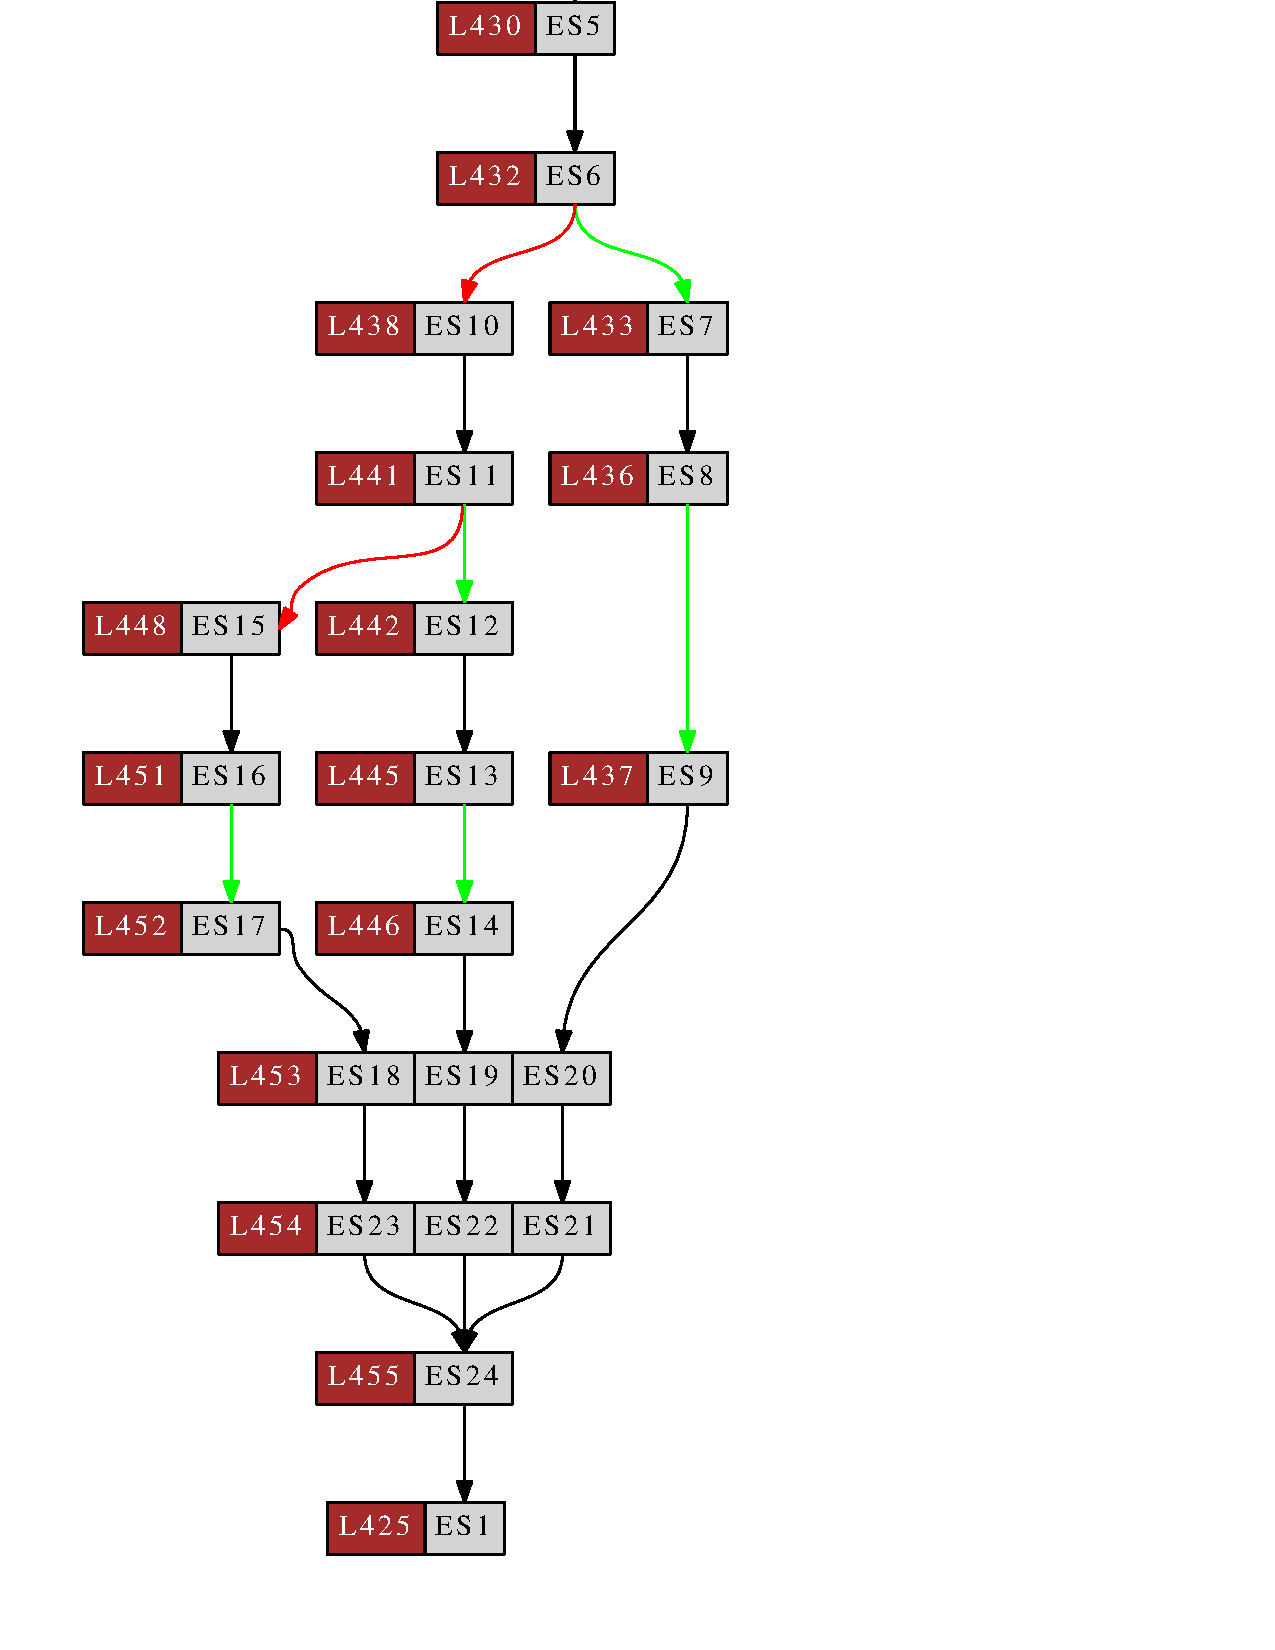
\includegraphics[width=0.7\textwidth]{gfx/basictest15_transitiongraph2.pdf}
\caption{Folded System State Transition Graph}
\end{figure*}

\begin{figure*}[t]
\centering
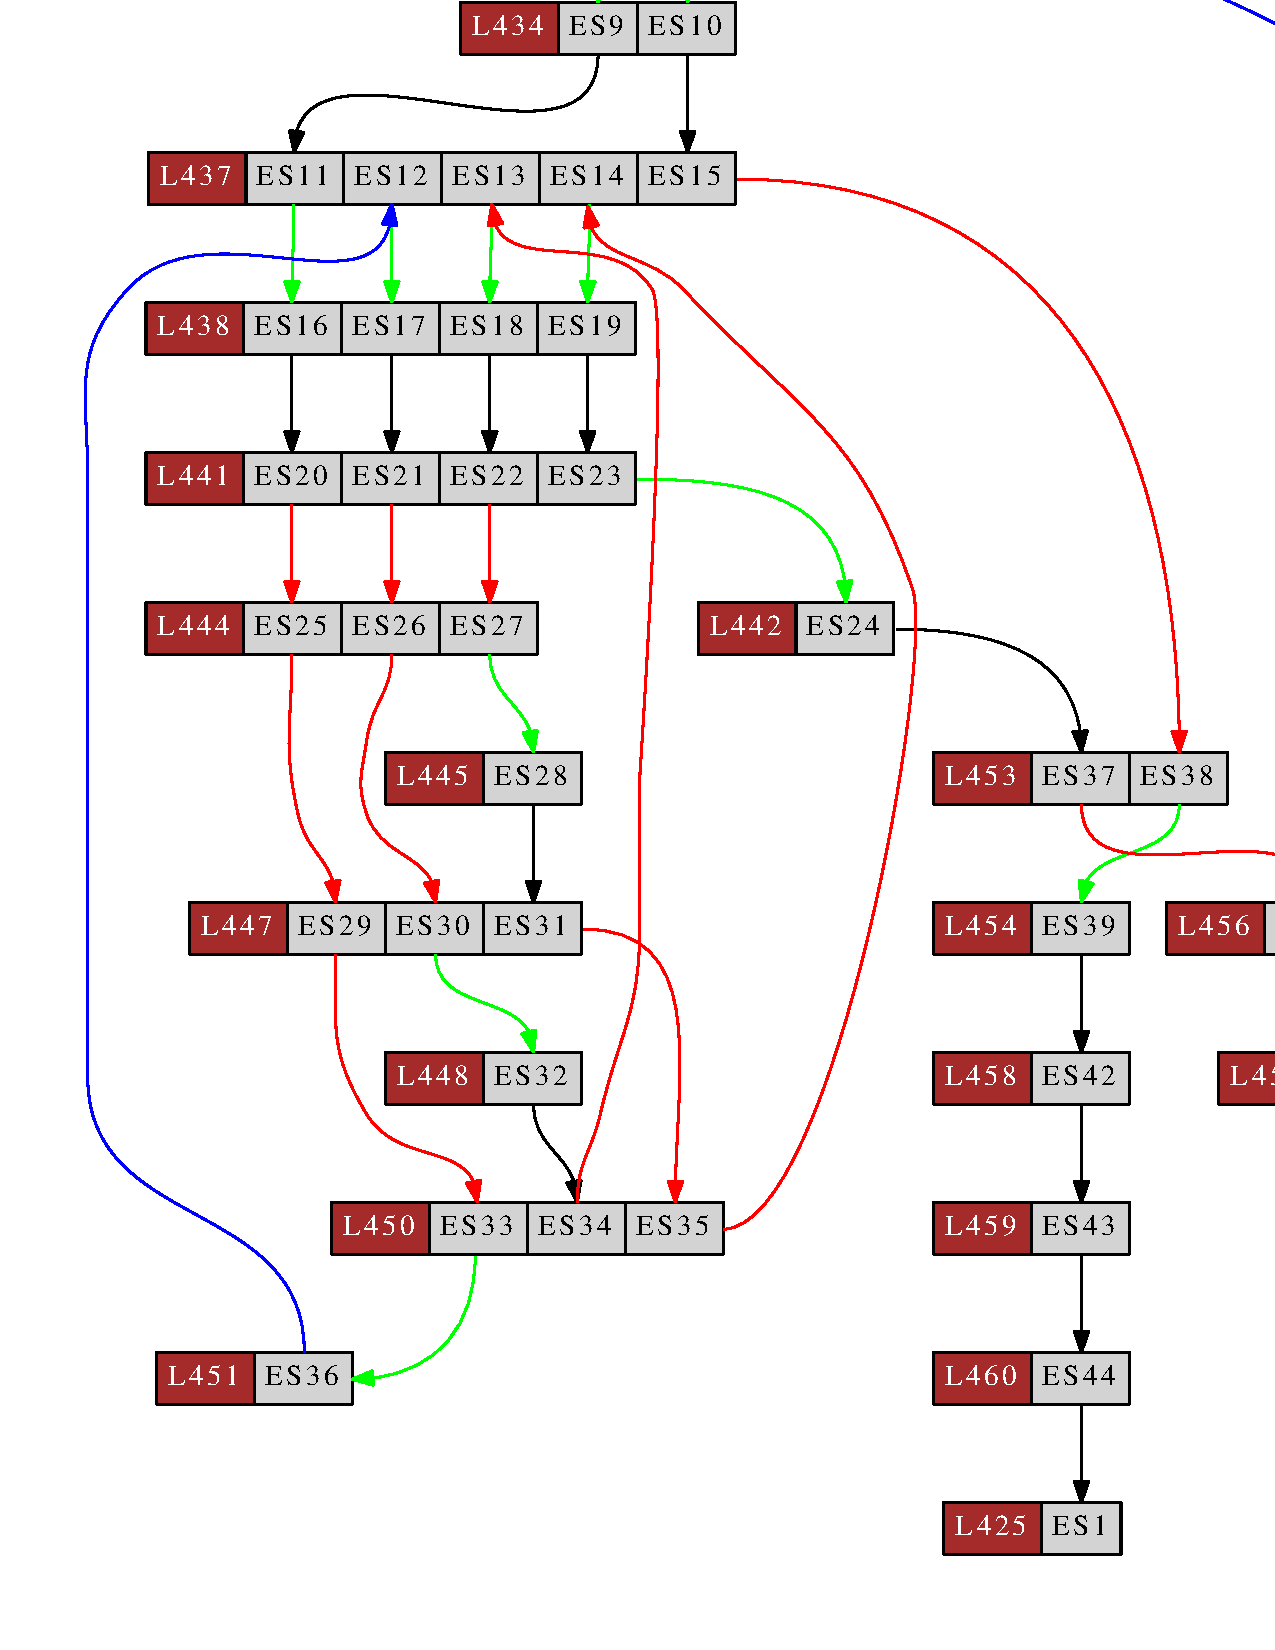
\includegraphics[width=0.7\textwidth]{gfx/basictest10f_transitiongraph2.pdf}
\caption{Folded System State Transition Graph (needs to reduced in size)}
\end{figure*}

\clearpage
\subsection{Property States}

\fixme{describe property states, const-int-lattice}

\subsection{Minimal Constraint Sets}
A minimal constraint set (MCS) is a minimal representation of
information about the values of variables and relations beetween the
variables with a minimal number of operators. The minimal number is
important for using a minimal amount of memory and for a proper
sorting criteria to be used in a sorted data structure.

The operators can range on variables and constants. Let x,y,z denote variables, and c, d constants with c!=d.
The constraints of interest are : 
\begin{itemize}
\item $x\eq c$: const-equality constraint
\item $x\neq c$, const-inequality constraint
\item $x\eq y$, var-equality constraint
\item $x\neq y$, var-inequality constraint
\end{itemize}

Additionally a set can be marked to represent an disequality, meaning that an equality and an inquality on the same variable have been added to the set. This is represented as \{\#\#\}.

Set union of MCS1 and MCS2 means inserting one constraint after another of MCS2 into MCS1.

The empty constraint set is minimal.

We define the consistency of a MCS by definining the effect of adding a new constraint to a set and define all cases.
Secondly, as we shall see, to maintain consistency, we also need to define effects for removing a constraint.

\fixme{rewrite to be become more concise}

1) Adding constraints to a MCS:

Adding a constraint C to an empty MCS gives a MCS.

\[\{\}+\{x=c\}\rhd \{x=c\}\]
\[\{\}+\{x\neq c\}\rhd \{x\neq c\}\]
\[\{x=c\}+\{x=c\}\rhd \{x=c\}\]
\[\{x=c\}+\{x=d\}\rhd \{\deqop\} with c<d\]
\[\{x=c\}+\{x\neq c\}\rhd \{\deqop\}\]
\[\{x\neq c\}+\{x=c\}\rhd \{\deqop\}\]
\[\{x\neq c\}+\{x\neq d\}\rhd \{x\neq c,x\neq d\}\]
No operations are defined on a MCS which includes a \{\deqop\} constraint.
\[\{x\neq c\}+\{x=d\}\rhd \{x=d\}\] (we drop the inequality on x)
\[\{x\neq c\}+\{x=d\}\rhd \{x\neq c,x=d\}\]
Lemma1: for each variable there can exist at most one const-equality constraint $x=c$.
Lemma2: if there exists a const-equality constraint for variable x, no const-inequality constraints can exist for this variable (and any other variable which is equal to that variable, i.e. an y=x constraint exists).
\[\{\}+\{x=y\}\rhd \{x=y\} if lex(x)<lex(y)\]
\[\{\}+\{x=y\}\rhd \{y=x\} if lex(x)\geq lex(y)\]

the rhs argument of '+' is sorted such that:
\[x=y \rhd  x=y if lex(x)<=lex(y)\]
\[x=y \rhd  y=x if lex(x)>lex(y)\]

\[\{x=y\}+\{x=c\}\rhd \{x=y,x=c\}\]
\[\{x=y\}+\{x\neq c\}\rhd \{x=y,x\neq c\}\]
\[\{x=y\}+\{y=c\}\rhd \{x=y,x=c\}\]
\[\{x=y\}+\{y\neq c\}\rhd \{x=y,x\neq c\}\]

\[add(MCS,\{x=y\})\rhd \{\deqop\} if constants(x,MCS)\neq constants(y,MCS)\]
\[add(MCS,\{x=y\})\rhd MCS+\{x=y\} if constants(x,MCS)=constants(y,MCS)\]

2) Removing constraints from an MCS:
\[remove(MCS,\{x\neq c\})\rhd MCS-\{x\neq c\}\]
\[remove(MCS,\{x=c\})\rhd MCS-\{x=c\}\]
remove($MCS,\{x=y\}$)$\rhd$  (lazy reorganization of constraint set)\\
  if(constraintexists($x,MCS\backslash\{x=y\}$) and constraintexists($y,MCS\backslash\{x=y\}$)\\
     $\rhd$  moveconstconstraints($x,y,MCS)\backslash\{x=y\}$)\\
  if(constraintexists($x,MCS\backslash\{x=y\}$) and not constraintexists($y,MCS\backslash\{x=y\}$)\\
     $\rhd$  moveconstconstraints($y,x,MCS)\backslash\{x=y\}$)\\
  if(not constraintexists($x,MCS\backslash\{x=y\}$) and not constraintexists($y,MCS\backslash\{x=y\}$)\\
     $\rhd$  $MCS\backslash\{x=y\}$\\
remove($MCS,\{x\neq y\}$) $\rhd$ $MCS-\{x\neq y\}$\\

We move all const-constraints of one variable to the other in case x=y was the last constraint concerning this variable. If no constraint remains for both variables (case 3), we can savely remove the x=y constraint.

We could achieve also a canonical representation if the moving of constraints would be performed when adding constraints (note that we order $x=y$ constraints according to the lexical order of x,y).

Auxiliary functions:
lex(x) : we use the ids as order criteria 
constraintexists(x,MCS) : constraint with this variable exists
constants(x,MCS) : number of constants that can be computed for this variable

\fixme{move to more prominent location}

Data Representation:
PState = Var x Val where Val is either a constant or top. Val is a lifted integer set.
SState = Lab x PState x Constraints x IO

Constraints is a set of constraints (see above).

IO determines whether one of the variables in PState is an input or output variable. More specifically, whether a variable is read from stdin, or printed to stdout or stderr. Furthermore it determines whether the state produces an output which is caused by a failed assert.


Labels are unique and represented as numbers. Ordering is therefore the same as for numbers.

IO is ordered by the variable it is concerned of and by the internal number that is associated with the IO-operation.

Each constraints set is associated with an id. The id is used in PState.

Hence, the analysis information is represented as:

\begin{itemize}
\item Label: num
\item PState: set of VarId x ValId
\item SState: set of Label x PStateId x ConstraintId x IOId
\end{itemize}

\subsection{Input/Output and Exit Information}

\section{Solver}

\fixme{describe algorithm}

\section{Implementation}

\fixme{describe data organization, approach for reducing redundancy, etc.}

A PState is sorted by the lexical order of the variables.
PState$\eq$ PState: two PStates are equal if all variable bindings are equal.
PState$<$ one PState is smaller than another if, considering the sequence of variables as a string, the string is smaller than the other according to lexical order.

% !TEX root = codethorn.tex
\section{Verifying LTL formul\ae}

\newcommand{\ffalse}{\ensuremath{\mathit{false}}}
\newcommand{\ttrue}{\ensuremath{\mathit{true}}}

At its heart CodeThorn uses a dataflow-based approach to verify LTL
formul\ae\ on the State Transition Graph. The algortihm consists of
two layers. At the outer layer, the abstract syntax tree of the
formula is traversed in bottom-up order. Every subexpression of the
LTL formula found by the traversal is reduced to a single value in the
Boolean lattice (\cf Fig.~\ref{fig:bool_lattice}) for each state in
the State Transition Graph . This evaluation is performed using a
dataflow analysis, which represents the inner layer of the alorithm.

\begin{figure}
  \centering
   \begin{tikzpicture}[scale=.9]
    \small
    \node (top) {$\top$} 
    child {node (-1)    {\ffalse}}
    child {node (0)     {}
      edge from parent[draw=none]
      child {node (bot) {$\bot$} 
      edge from parent[draw=none]
      }
    }
    child {node (1)    {\ttrue}} 
    ; 
    \draw (-1)    -- (bot);
    \draw (1)     -- (bot);
  \end{tikzpicture} 
  \caption{Boolean lattice the LTL formul\ae are reduced to}
  \label{fig:bool_lattice}
\end{figure}

\newcommand{\state}{\ensuremath{\mathit{s}}}
\newcommand{\STG}{\ensuremath{\mathrm{STG}}}
\newcommand{\States}{\ensuremath{\mathit{States}}}
\newcommand{\prop}[1]{\ensuremath{p_{\state,#1}}} 
\newcommand{\propp}[1]{\ensuremath{p_{\state',#1}}} 
\newcommand{\G}{\ensuremath{\mathrm{G}}}
\newcommand{\F}{\ensuremath{\mathrm{F}}}
\newcommand{\X}{\ensuremath{\mathrm{X}}}
\newcommand{\R}{\ensuremath{\mathrm{R}}}
\newcommand{\U}{\ensuremath{\mathrm{U}}}
\newcommand{\WU}{\ensuremath{\mathrm{WU}}}

The remainder of this section will discuss how the transfer functions
for each element of the LTL grammar are defined. We are using the
following notational conventions. The
$\STG={\mathit{States},\mathit{Transitions},\mathit{Start}}$ is the
(reduced) State Transition Graph (or Kripke Model
\citep[pg. 27ff]{Clarke1999}). For each state \state\ we have an array of $n$
properties \prop{i}, $i \in [0\dots n]$, where $n+1$ is the number of
sub-expressions in the LTL formula.

\subsection{Boolean Operators: \texttt{!}, \texttt{\&}, \texttt{|}}
The boolean operators in LTL have the least computationally complex
transfer functions as their effect is only local.
\begin{align*}
e &= !a  & \forall\state\in\States\colon\prop{e} &:= \neg\prop{a}\\
e &= a \& b & \forall\state\in\States\colon\prop{e} &:= \prop{a} \cap \prop{b}\\
e &= a | b & \forall\state\in\States\colon\prop{e} &:= \prop{a} \cup \prop{b}\\
\end{align*}

\subsection{The G operator}
The global operator $\G a$ yields true iff the subexpression $a$ is true at
all states.

\[ e = \G a \qquad \forall\state\in\States\colon\prop{e} :=\bigcap_{\state\prime\in\States}{\propp{a}} \]

\subsection{The X operator}
The next operator $X a$ yields true iff $a$ is true in the next state.
\[ e = \X a \qquad\forall\state\in\States\colon\prop{e}:=\bigcap_{\state\prime\in succ(\state)}{\propp{a}} \]

\subsection{The operators F, R, U, and WU}
These operators are computationally more intensive, since we need to
perform a fix point search over the entire state transition graph. Backward.
\begin{tabular}{rlllll}
\toprule
operator & $\mathit{init}$ & $\mathit{start}$ & $\mathit{join}$ &
$\mathit{calc}$ & $\mathit{otherwise}$ \\\midrule

$e = \F a$  & $\ffalse$ & $(\prop{a}==true)$ & $\cup$ & 
$\prop{a}\cup\bigcup_{\state\prime\in succ(\state)}{\prop{e}}$ &\\

$e = a \R b$ & $\bot$ & $(\prop{b}==true)$ & $\cap$ &
$\prop{b} \cap \prop{a} \cup \bigcap_{\state\prime\in succ(\state)}{\prop{e}}$\\

$e = a \U b$ & $\ffalse$ & $(\neg\prop{b}==bot)$ &
$\cup$ & $\prop{a} \cup\bigcap_{\state\prime\in succ(\state)}{\prop{e}}$ & $\ffalse$\\

$e = a \WU b$ & $\bot$ & $(\prop{a}==true)$ & $\cup$ &
$\prop{a} \cup \bigcup_{\state\prime\in succ(\state)}{\prop{e}}$\\\bottomrule
\end{tabular}


\subsection{Handling I/O nodes}
\begin{itemize}
\item are propagated to the next I/O state of the same type
\end{itemize}

\subsection{Reducing the State Transition Graph}

\subsection{Debugging: Finding counterexamples}

\bibliographystyle{unsrtnat}
\bibliography{codethorn}

\end{document}
